\chpt{A two-part mixed-effect model for analyzing longitudinal microbiome compositional data} \label{chpt4:ZIBR}


In this Chapter, a statistical model is proposed for longitudinal microbiome data analysis. Longitudinal measurements of microbial communities are commonly obtained in many microbiome studies. A key question in such microbiome studies is to identify the microbes that are associated with clinical outcomes or environmental factors. However, the longitudinal microbiome compositional data are highly skewed, bounded in [0,1), and often sparse with many zeros. In addition, the observations from repeated measures are correlated. A method that takes into account these features is needed for association analysis in longitudinal microbiome data. In this chapter, we propose a two-part zero-inflated Beta regression model with random effects (ZIBR) for testing the association between microbial abundance and clinical covariates for longitudinal microbiome data. The model includes a logistic regression component to model presence/absence of a microbe in samples and a Beta regression component to model non-zero microbial abundance, where each component includes a random effect to take into account the correlations among repeated measurements on the same subject. Both simulation studies and the application to real microbiome data show that ZIBR model outperforms the previously used method. This provides a useful tool for identifying the relevant taxa based on longitudinal or repeated measures in microbiome research.
The model was implemented in R package ZIBR and freely available at https://github.com/chvlyl/ZIBR.



\section{Introduction}
The human microbial communities are associated with many human diseases such as obesity, diabetes and inflammatory bowel disease (IBD) \citep{turnbaugh2006obesity, qin2012metagenome, Kostic:2015bh}. In order to decipher the function and impact of the microbes on the human well-being, two high-throughput sequencing based approaches have been widely used in microbiome studies. One is the 16S ribosomal RNA (rRNA) sequencing approach, which profiles bacterial community by sequencing the 16S rRNA marker gene. Another approach is the shotgun sequencing, which sequences all the microbial genomes presented in the sample, rather than just one marker gene. Both 16S rRNA and shotgun sequencing approaches are quite useful and have been widely applied to human microbiome studies, such as the Human Microbiome Project (HMP) \citep{turnbaugh2007human} and the Metagenomics of the Human Intestinal Tract (MetaHIT) project \citep{qin2010human}. To quantify the microbial abundance, the sequencing reads usually are aligned to some known reference sequences \citep{segata2012metagenomic}. Due to the uneven total sequence counts of samples, the microbial abundance measured in read counts are not comparable across samples. Therefore, it is common that the read counts are normalized to the relative abundance by dividing total sequence counts in the sample so that the relative abundances of all microbes in one sample sum to one \citep{tyler2014analyzing}, resulting in compositional data with lots of zeros. 


It is of great interest to study how microbial abundance changes across time and its association with treatments, clinical outcomes or other covariates. To address this question, many microbiome studies employed the longitudinal study design (for reviews, see \cite{Faust:2015bd, Gonzalez:2012gv, Gerber:2014ca}). For example, \citet{lewis2015inflammation} studied the gut microbiome from pediatric IBD patients during an eight-week treatment. One interesting question in this study is to identify the bacterial taxa that change their abundance under different treatments across time. In another longitudinal microbiome study, \citet{Backhed:2015kc} studied the microbiome change during the first years of newborn babies with different delivery methods and feeding activities. 


Modeling such sparse longitudinal compositional data is challenging for several reasons. First, the microbiome compositional data is non-normally distributed and bounded in [0,1). Methods with normal distributional assumption are not expected to perform well. Second, the microbiome data is often observed with many zeros, which leads to great heterogeneity in the data. Third, in microbiome studies, it is important to adjust for the other covariates/confounders such as patient age or antibiotics use. Therefore, a multivariate regression based method is more preferred than univariate tests such as the t-test or Wilcoxon rank test. Fourth, the repeated measurements in the longitudinal data are correlated, i.e, observations from the same subject across time are not independent. This renders the methods with independence assumption not directly applicable. Ignoring the correlation among repeated measures can lead to incorrect inference. Therefore, taking into account the correlation among repeated measurements is necessary. 


Several methods have been used to analyze the longitudinal data in order to identify the covariate-associated taxa, but with their own limitations. To overcome the issue of non-independence of the data across time points, most of the longitudinal microbiome studies analyzed data at individual time point \citep{Cox:2014hy, arrieta2015early, Rutten:2015bx, Zhou:2015kw, David:2014cl, Schulz:2014fy} or compared two time points but ignored the other time points \citep{Backhed:2015kc, Koren:2012ji}. To take into account the excessive zeros in the data, a two-part test combining a Z-test for testing the proportion of zeros and a Wilcoxon rank-sum test for testing the non-zero values, was developed for identifying differential abundant microbes between two groups \citep{wagner2011application, markle2013sex}. Such tests cannot be applied to longitudinal correlated data and are limited to only two-group comparison. \citet{Romero:2014il} used a zero-inflated Poisson regression model with random effect to take into account the correlations in longitudinal data, but the model can only be applied to count data. A linear mixed effect model with arcsine square root transformation on the microbiome compositional data was used \citep{LaRosa:2014kk, Kostic:2015bh}, however, this method does not explicitly handle the excessive zeros in the data. This motivates us to develop a flexible method that identifies the covariate-associated taxa while handling the features of the microbiome compositional data and jointly modeling data from all time points. 


The focus of this chapter is to develop a statistical model for identifying the bacterial taxa that are associated with covariates while addressing the above limitations. We propose a two-part mixed-effect zero-inflated Beta regression model, which is a mixture of a logistic regression component and a Beta regression component, with the random effects included in the model to allow the correlations between repeated measures. This model takes into account the nature of the microbiome compositional data and also allows for multiple covariates in the regression setting. In addition, the model can jointly analyze data from all the time points. Simulation results show that our method outperforms several previously used methods in terms of increased power in detecting covariate-associated taxa. We apply ZIBR to a real microbiome study and identify several bacterial taxa that are associated with different treatments of inflammatory bowed disease (IBD). ZIBR model was implemented in R package ZIBR and is freely available at https://github.com/chvlyl/ZIBR.


\section{A two-part mixed-effect regression model for longitudinal microbiome data}
To illustrate the features of the sparse compositional data observed  in microbiome studies, Figure \ref{Fig1} shows the distribution of the relative abundance of two bacterial genera from a real microbiome data set from \citet{lewis2015inflammation}.  The data show several important features: (1)  are  bounded in [0,1);  (2) the data highly skewed; (3) the data include  excessive zeros.   In addition, if the microbiome data are measured in a longitudinal study, the repeated measures from the same subjects across time points are expected to be correlated.  In order to identify the microbes that are associated with clinical outcomes, we develop a two-part logistic-Beta regression model with random effects to model such longitudinal data. 

\begin{figure}[!tpb]%figure1
\centerline{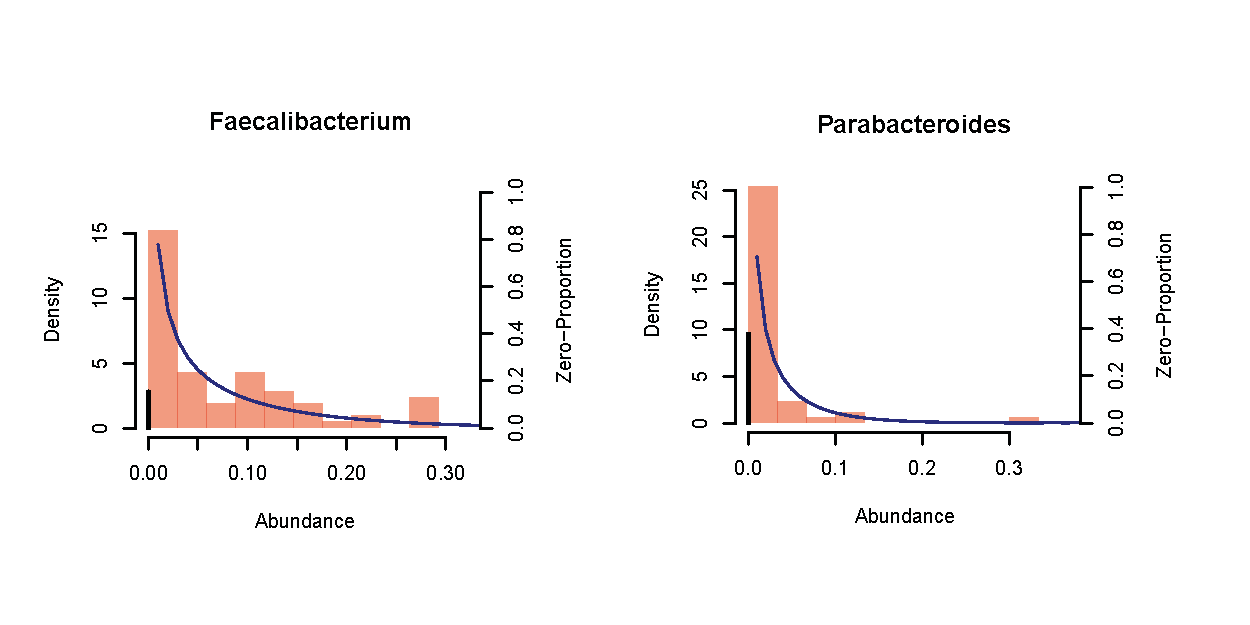
\includegraphics[scale=0.7,trim=0 40 0 0,clip]{Figure/F41_Distribution_of_Real_Data_v3.pdf}}
\caption[Examples of two genera from the real human microbiome data]{Examples of two genera from the real human microbiome data. Red bars represent the density of the non-zero data (left Y axis). Black bars represent the zero proportion (right Y axis). Back curves show  the fit of the non-zero data using a  Beta distribution.}
\label{Fig1}
\end{figure}

Our model considers each taxon separately. For each given bacterial taxon, let $Y_{it}~(i = 1,2,\ldots,N, t= 1,2,\dots,T)$ be its relative abundance for subject $i$ at time $t$, where $0 \le Y_{it} < 1$.   We assume that 
\begin{align}
Y_{it} &\backsim 0 \text{ with probability } 1-p_{it}\\
&\backsim \mbox{Beta}(\mu_{it}\phi,(1-\mu_{it})\phi) \text{ with probability } p_{it},
\end{align}
where the  density function of the Beta distribution is parameterized as
\begin{equation}\label{beta1}
f(y_{it};\mu_{it},\phi) = \frac{ \Gamma(\phi)}{ \Gamma(\mu_{it}\phi)\Gamma((1-\mu_{it})\phi)}y_{it}^{\mu_{it}\phi-1}(1-y_{it})^{(1-\mu_{it})\phi-1}
\end{equation}
with $\mu_{it}$ $(0<\mu_{it}<1)$ and $\phi$ $(\phi>0)$ being  the mean and dispersion parameters of the Beta distribution, respectively. The parameter $p_{it}$ is the probability that the observation $Y_{it}$ is generated from the Beta component. Figure \ref{Fig1}  shows that the Beta distribution fits  the non-zero values of the real data well.  In addition,  we let the probability $p_{it}$ of the logistic component and the mean of the Beta component $\mu_{it}$ depend on the covariates through the logit link function,
\begin{align}
\mbox{logit}(p_{it})&= \log\left(\frac{p_{it}}{1-p_{it}}\right) = X_{it}^T \alpha + a_i,\label{logit1}\\ 
\mbox{logit}(\mu_{it})&= \log \left(\frac{\mu_{it}}{1-\mu_{it}}\right) = Z_{it}^T \beta + b_i,\label{logit2}
\end{align}
where $a_i$ and $b_i$ are the individual-specific random intercepts,  $X_i$ and $Z_i$ are the covariates that can be time-dependent and are  not necessarily  the same, and $\alpha$ and $\beta$ are the corresponding vectors of the regression coefficients. 

This model can be considered as a two-part model with a logistic component and a Beta component. The logistic component  models the presence/absence of the taxon in the samples and the Beta component  models the non-zero abundance of the taxon.  A covariate can  affect the microbiome composition  in two different   ways: (1) it  affects the presence/absence of the taxon in the samples, which is modeled through the logistic regression part in the model; (2) it affects the relative abundance when the taxon presents in the samples. This is modeled by the Beta regression in the model. The data observed are from  a mixture of these two models.  This model is flexible to allow  that the covariates affecting  the presence/absence of the microbial species and the covariates affecting  microbial abundance to be different. 

If the data are measured at repeated times, the responses at different time points within a subject are expected to be correlated. The repeated measures $Y_{it}$ ($t=1,\ldots,T)$ on the same subject $i$ share the same individual-specific values of $a_i$ and $b_i$, which can be used to model such correlations.  We only include the random intercepts in the model since such  simple random intercepts are often adequate in practice \citep{min2005random} to capture the longitudinal correlations.  However, it is easy to extend our model to include   random slops. The random effects are assumed to follow an independent normal distribution, 
\begin{align*}
a_{i}  \sim N(0,\sigma_1^2), \quad 
b_{i} \sim N(0,\sigma_2^2).
\end{align*}


The parameters can be estimated by the standard maximum likelihood estimation (MLE), where  the likelihood function  is given as 
\begin{multline*}
L (\alpha,\beta, \phi, \sigma_1^2, \sigma_2^2)\\
= \prod_{i=1}^{N}\int_{-\infty}^{\infty}\int_{-\infty}^{\infty}  \prod_{t=1}^{T}(1- p_{it})^{I(Y_{it}=0)}[p_{it} f(\mu_{it},\phi)]^{I(Y_{it}>0)} \\
\times  g(a_i,b_i | \sigma_1^2,\sigma_2^2)\, \mathrm{d}a_i\mathrm{d}b_i,
\end{multline*}
where $p_{it}$ and $\mu_{it}$ are defined through the logistic regression models \eqref{logit1}-\eqref{logit2},  $f(\mu_{it},\phi)$ is the Beta density function given in \eqref{beta1} and $g(a_i,b_i | \sigma_1^2,\sigma_2^2)$  is  the product of two normal density functions. 

To evaluate this likelihood function, we first integrate out the unobserved random effects to obtain a marginal likelihood. Since the integrals are analytically intractable, the marginal likelihood does not have a closed-form. We use Gauss-Hermite quadrature to approximate the integral by a finite sum. The MLE of   $(\alpha, \beta, \phi, \sigma_1^2, \sigma_2^2)$ can be obtained numerically.
We use likelihood ratio test  for three  biologically interesting  null hypotheses:
\begin{enumerate}
\item  the covariates are associated  with the bacterial taxon  by affecting its presence or absence, 
$H_0: \alpha_j = 0$; 
\item the taxon  is associated with the covariates by showing different abundances, $H_0:\beta_j = 0$;
\item  the covariates affect the taxon   both in terms of presence/absence and its abundance, $H_0:\alpha_j=0~ and~ \beta_j=0$ for each covariate $X_j$ and $Z_j$.
\end{enumerate}
The $p$ values can be obtained for each of these hypotheses. If the covariate $X$ and $Z$ are the same,  the joint  null is $H_0:\alpha_j=0$ and $\beta_j=0$, which tests the overall association between the covariate and the taxon abundance.  We have implemented this model as an  R package {\it ZIBR}. 



\section{Simulation studies}
To evaluate the performance of our proposed method ZIBR for longitudinal microbiome data, we carried out simulation studies first. We compared our method with linear mixed effect model with arcsine squared root transformation (LMM) on the microbiome abundance as proposed in \cite{LaRosa:2014kk} and \cite{Kostic:2015bh}. We compared ZIBR with LMM since  it was currently the only method that can jointly model data measured over all time points in  longitudinal microbiome studies. 

We first evaluated the type I errors of the two methods. The simulation was carried out with different number of subjects ($N=50,100,150$), each with $T=5$ time points. One binary covariate for both logistic and Beta components was used to mimic the case-control study design, where $X=Z=0$ for $\frac{1}{2}N$ subjects and $X=Z=1$ for the other $\frac{1}{2}N$ subjects. We set the regression coefficients as $\alpha = (0,0)$, $\beta = (-0.5,0)$, the variance of the mixed effect as $\sigma_1 = \sigma_2 = 0.5$ and the dispersion parameter of the Beta distribution as $\phi=5$. These parameters were chosen to mimic parameters estimated based on the real data analyzed in Chapter~\ref{chpt2:please}. The simulations were repeated 10,000 times under each sample size setting. The type I error was calculated with two different nominal levels of 0.001 and 0.05.

The results are shown in Table~\ref{zibrtypeIerror}, indicating that both our proposed method ZIBR and LMM control the type I error reasonably well. We also evaluated  the running time of ZIBR. It took 2.3s, 4.0s, and 7.0s per simulation  to run on a Macbook Pro laptop for sample size of  $N$=50, 100, 150, respectively, indicating that the algorithm is very efficient. 





\begin{table}[t]
\begin{center}
\caption[Type I error for ZIBR and LMM]{Type I error for ZIBR and LMM for $\alpha$-level of 0.05 and 0.001 for various sample sizes. Simulations were repeated 10,000 times.}\label{zibrtypeIerror}
{\begin{tabular}{lcccc}\toprule
& ZIBR & LMM & ZIBR & LMM \\
\cline{2-3}\cline{4-5}
Sample size 	& \multicolumn{2}{ c }{0.001}&\multicolumn{2}{ c }{0.05}\\

$N$=50   &0.013 & 0.0107 & 0.0584 &	0.0484\\
$N$=100  &0.0105 &	0.0096 & 0.0532 &	0.0507\\
$N$=150  &0.0095&	0.001&0.0493	&0.0494\\
\bottomrule
\end{tabular}}{}
\end{center}
\end{table}



We next simulated the data sets to evaluate the power of  ZIBR for identifying  the true association. We simulated 1000 bacterial species, of those, 400 were associated with a binary covariate and the rest, 600, were not associated.  For each species, we simulated $N$=50 subjects with $T$=5 time points for each subject. We simulated the regression coefficients $(\alpha_0,\alpha_1,\beta_0,\beta_1)$ either from a uniform distribution  or set them to zero. Particularly,  they were set to  (1)  $(-0.5, U(0.1,1), -0.5,  U(0.1,1))$ for 100 species; (2) $(0.5, U(-1,-0.1), 0.5,  U(-1,-0.1))$  for 100 species; (3)  $(-0.5, U(0.1,1), 0.5,  U(-1,-0.1))$ for 100 species; (4) 
$(0.5, U(-1,-0.1), -0.5,  U(0.1,1)$ for 100 species; (5) $(0, 0, -0.5, 0)$ for 600 species.  Here scenarios (1) and (2) indicate that the association in the logistic and Beta components have the same direction while scenarios (3) and (4) indicate different directions. Scenario (5) indicates no association  in either logistic or Beta component. We simulated variance of the random effect as $\sigma_1 \sim U(0.1, 1)$, $\sigma_2 \sim U(0.1, 1)$  and Beta dispersion parameter as $\phi \sim U(2,10)$. The performance of ZIBR and LMM were evaluated based on the ROC curve for identifying the covariate-associated species. The ROC and AUC analysis were performed using pROC package in R \citep{Robin:2011fc}. 
The results are shown in Figure \ref{Fig2}.
The AUC for ZIBR is 92.0 compared to 79.1 for LMM, showing a significant difference  ($p< 2.2 \times 10^{-16}$ by DeLong's test). 

\begin{figure}[!tpb]%figure2
\centerline{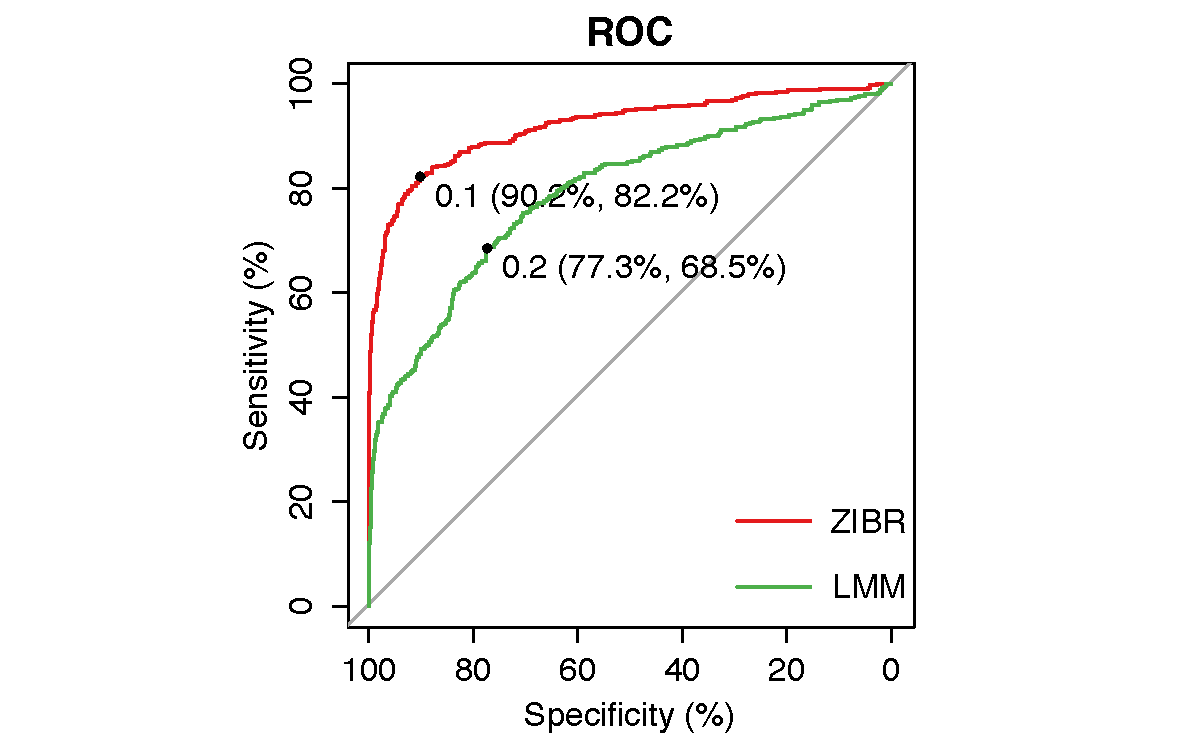
\includegraphics[scale=0.8,trim=0 0 0 0,clip]{Figure/F42_ROC.pdf}}
\caption[ROC curves for identifying association by ZIBR and LMM]{ROC curves for identifying association by ZIBR and LMM, where 1000 species were  simulated and 400 of them had true association with the covariate. The simulations were carried out with $N=50$ subjects and $T=5$ time points for each subject. LMM is the linear mixed effect model with arcsine squared root transformation on the microbial abundance. The best cutoff and the corresponding specificity and sensitivity for each method are indicated, where the best cutoff is defined as the value such that the sum of sensitivity and specificity is the largest.}
\label{Fig2}
\end{figure}

\section{Real data analysis}
We applied ZIBR to a real microbiome study comparing different therapies for pediatric IBD patients \citep{lewis2015inflammation,lee2015comparative}. The study  collected 90 children  with IBD who received one of the three study therapies, including 52 children receiving anti-TNF,
22 receiving exclusive enteral nutrition (EEN) and  16 receiving partial enteral nutrition
with ad lib diet (PEN). Adequate stool samples were available from 86 individuals to
conduct shotgun metagenomic analysis. Gut microbiome samples were
collected at four time points: baseline, 1 week, 4 weeks, and
8 weeks into the therapy.  The bacterial abundances at genus level were  quantified using MetaPhlAn 1.7.6 \citep{segata2012metagenomic}. The low sequencing depth samples and low abundant genus were removed as in \cite{Kostic:2015bh}, \cite{Romero:2014il} and \cite{Stein:2013dl}. After filtering, we had a total of 236 samples with  59 subjects (47 anti-TNF and 12 EEN) and four  time points for each subject as well as 18 most common bacterial genera. Our goal was to identify the bacterial genera that showed overall different abundances over  three time points between  EEN and anti-TNF treatments, adjusting for time effect  and the  abundance at the baseline.  We fitted ZIBR with the baseline abundance, week and treatment as covariates and compared the results  from fitting the linear mixed effect model   \citep{LaRosa:2014kk,Kostic:2015bh} with the same covariates and a subject-specific random effect.   For the LMM, the relative abundance was arcsine squared-root transformed before fitting the model. The linear mixed effect model was fitted using the $lme$ function from $nlme$ package in R. The $p$-values were adjusted using  the Benjamini-Hochberg procedure to control the FDR.  



%%%-------------------------------------------------%%%
%%%------------------------Results------------------%%%
%%%-------------------------------------------------%%%

\begin{table*}[tb]
\begin{center}
\caption[Comparison of results between ZIBR and LMM for four bacterial genera]{Comparison of results between ZIBR and LMM for four bacterial genera, where three covariates, including the baseline abundance, time and treatment, are included in each model. For each genus, the FDR-adjusted $p$-value is shown for each of the three covariates in the model. }\label{tbl2}
\begin{tabular}{lcccccc}
\hline
\multicolumn{1}{l}{} & 	\multicolumn{3}{c}{LMM} & 		\multicolumn{3}{c}{ZIBR}\\		
Species	 &Baseline	&Time	&Treatment &	Baseline&	Time&	Treatment\\
\hline
Lactobacillus&	1.10E-11	&5.68E-02	&4.97E-01	&2.46E-07	&5.38E-01	&9.41E-03\\
Veillonella	&9.04E-07	&8.04E-01	&5.27E-01	&4.81E-07	&9.89E-01	&1.76E-02\\
Collinsella	&2.28E-07	&9.85E-01	&2.91E-01	&6.14E-09	&5.38E-01	&1.57E-02\\
Eubacterium&	1.03E-02&	1.84E-02&	5.04E-02&	1.18E-02&	2.43E-01&	2.67E-02\\
\hline
\end{tabular}
\end{center}
\end{table*}

At FDR=5\%, LMM identified  seven genera, including {\it Ruminococcus}, {\it  Faecalibacterium},  {\it Bifidobacterium}, {\it Dialister}, {\it  Streptococcus}, {\it  Haemophilus} and  {\it  Alistipes}. ZIBR identified all those seven genera and also identified four additional genera, {\it Lactobacillus, Veillonella, Collinsella}, and {\it Eubacterium} (see Figure~\ref{ZibrVenn}). Table \ref{tbl2} shows the FDR-adjusted $p$-value  for each of the three covariates in the model, indicating that the initial abundance of these four genera had large effects for their abundance during the course of the treatment. However, these genera were relatively stable in their abundance during the 8 weeks of treatments. 

After adjusting the baseline abundance, these four genera showed different abundances between anti-TNF and the EEN treatments. 
Figure~\ref{Fig4} shows the abundances of those four genera over time.  {\it Lactobacillus} and {\it Veillonella} were observed more frequently  in the anti-TNF treated group across  different time  points than in the EEN group.  However, no significant difference was observed for the  non-zero abundance when they were observed.   
In contrast, {\it Collinsella} and {\it Eubacterium}  showed  consistent differences across  all three time points in the non-zero abundance but not the frequencies being observed.   Results from ZIBR showed that different treatments led to different  probabilities of observing  {\it Lactobacillus} and {\it Veillonella} (FDR adjusted $p$=0.0049, FDR adjusted $p$=0.0085), but  not   {\it  Collinsella} and {\it Eubacterium} (FDR adjusted $p$=0.299,FDR adjusted $p$=0.50).  In addition, different treatments seemed to  lead to different abundances for  {\it Collinsella} and {\it Eubacterium} (FDR adjusted $p$=0.0254,FDR adjusted $p$=0.0254), but not for  {\it Lactobacillus} and {\it  Veillonella} (FDR adjusted p=0.42, FDR adjusted p=0.93). The advantage of ZIBR is that it considers these two types of differences simultaneously and therefore potentially leads to more power in detecting the differences in abundances between the two treatment groups. 


\begin{figure}[!tpb]%figure3
\centering{\includegraphics[scale=0.6,trim=20 120 85 150,clip]{Figure/F43_Treatment_Venn.pdf}}
\caption[Bacterial genera that showed  different abundances between anti-TNF and EEN treatments  identified by  ZIBR and LMM]{Bacterial genera that showed  different abundances between anti-TNF and EEN treatments  identified by  ZIBR and LMM after adjusting for the initial abundance.  LMM identified seven genera, which were  also identified by ZIBR. ZIBR  identified additional four genera.}
\label{ZibrVenn}
\end{figure}



\begin{figure}[!tpb]%figure4
\centerline{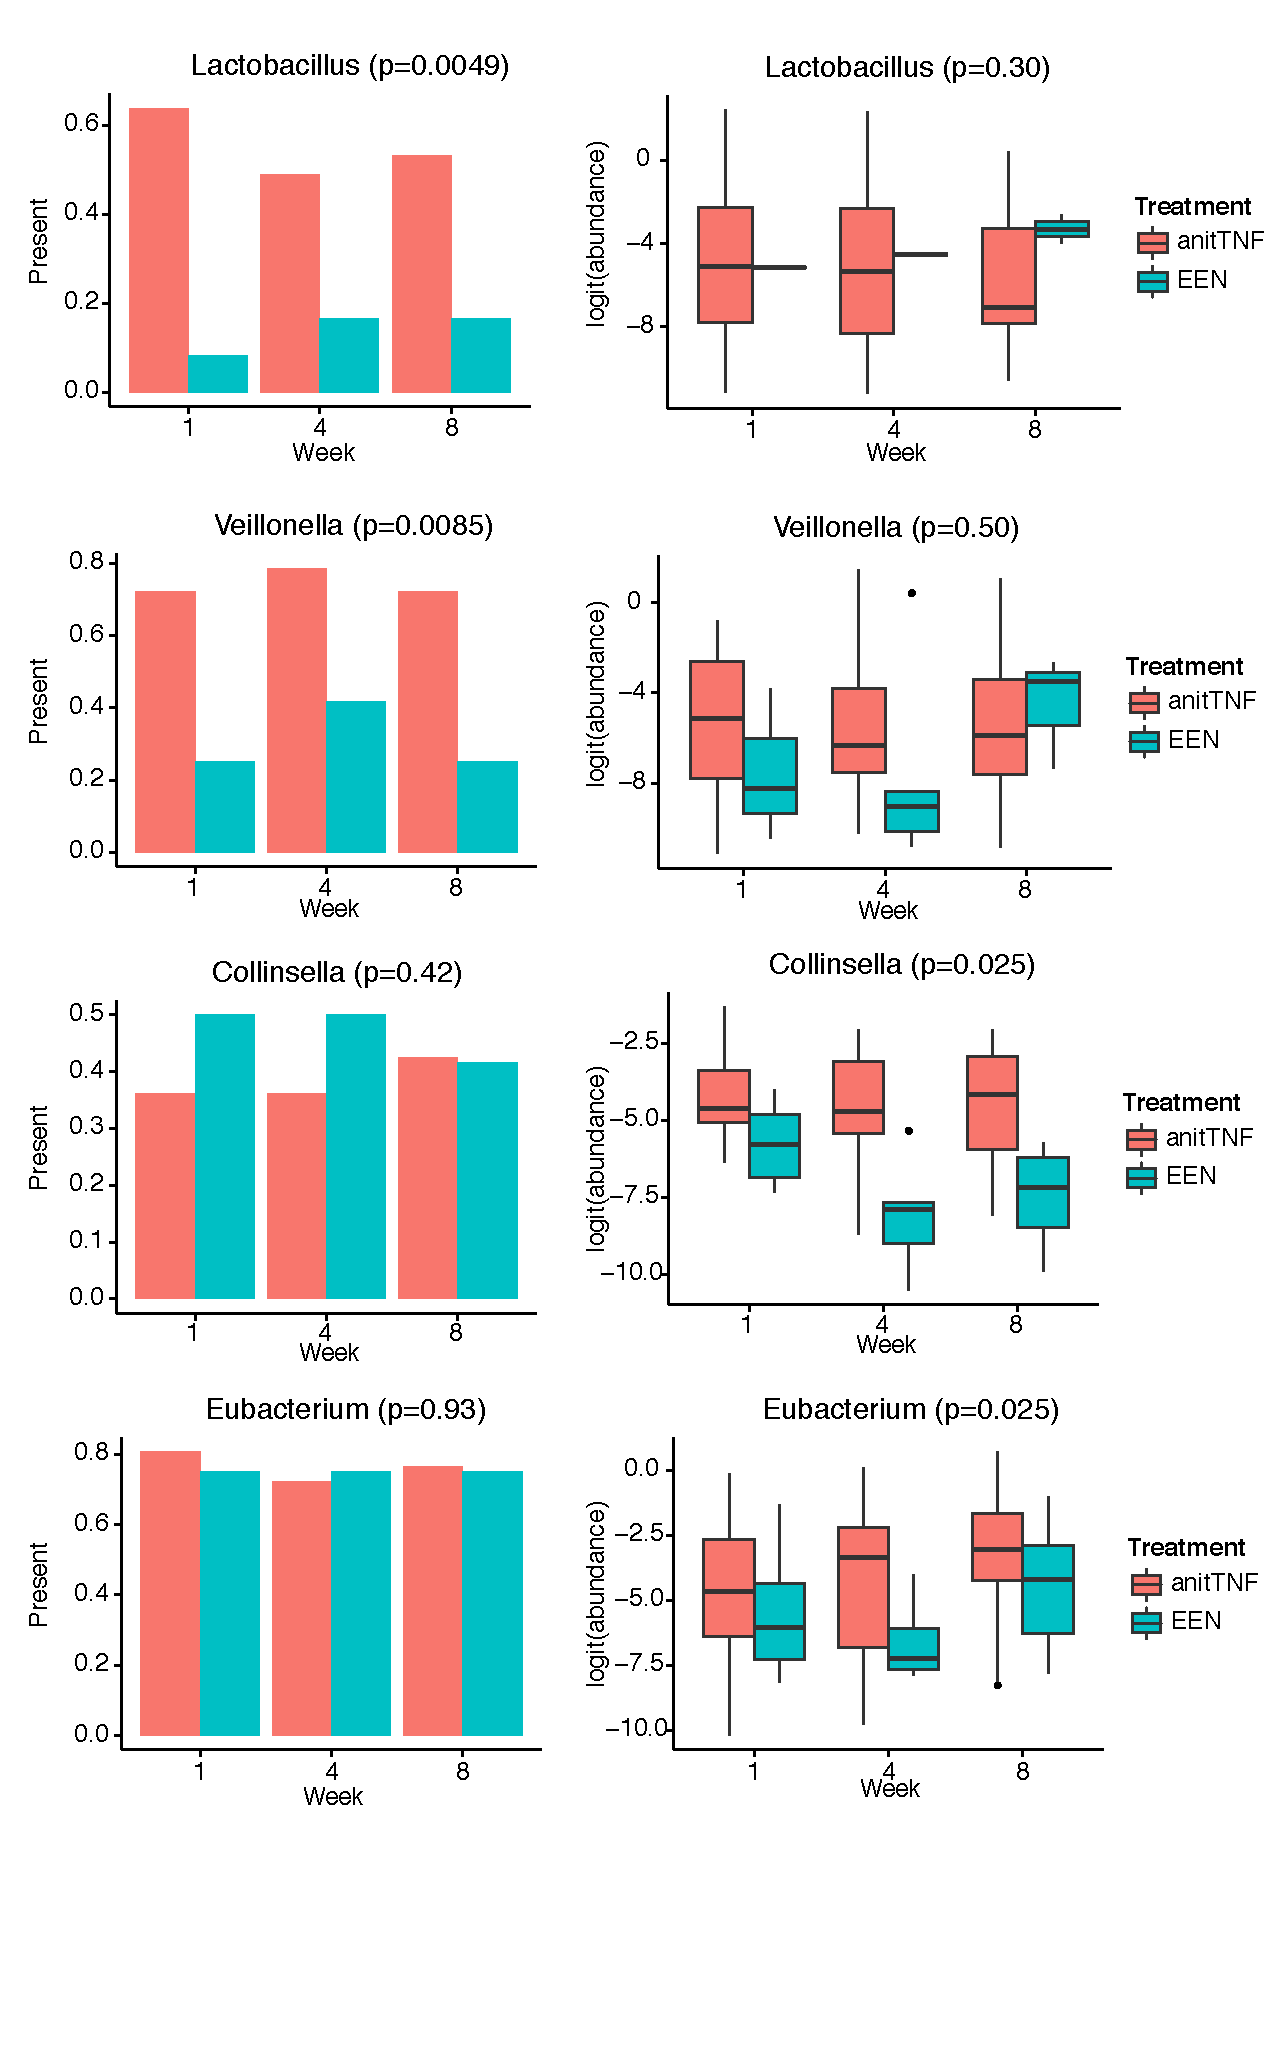
\includegraphics[scale=0.6,trim=0 120 0 0,clip]{Figure/F44_ZIBR_Three_Extra.pdf}}
\caption[Four  genera identified by ZIBR but not by LMM]{Four  genera identified by ZIBR but not by LMM. Left panel shows the percentage of samples in EEN or anti-TNF  groups where the  genus was present. Right panel shows the non-zero abundance in EEN or anti-TNF groups, where the abundances were logit-transformed.}
\label{Fig4}
\end{figure}


\section{Discussion}
We have proposed a two-part mixed-effect model to identify the taxa that are associated with clinical covariates in the longitudinal microbiome studies. Our model takes into account the compositional and sparse nature of the microbiome data as well as the correlation between repeated measures in the longitudinal study.  We  have demonstrated that our proposed model outperforms the commonly  used  linear mixed-effect models.  We  applied our method to the real human microbiome study of  IBD treatment  and identified a number of bacterial genera  that showed different abundances between two commonly used treatments during the eight-week treatment period. 

In our simulations  and analysis of real data, te ZIBR model  involves the same covariates for logistic regressions and Beta regression.  However, our model is more flexible, which  can include  multiple   covariates and different covariates  in two different  components of the model.  Besides identifying bacterial taxa, the model proposed here can also be applied  to identify microbial genes or pathways that show different profiles  in longitudinal microbiome studies.
